\begin{figure}[h!]
	 \centering 
	 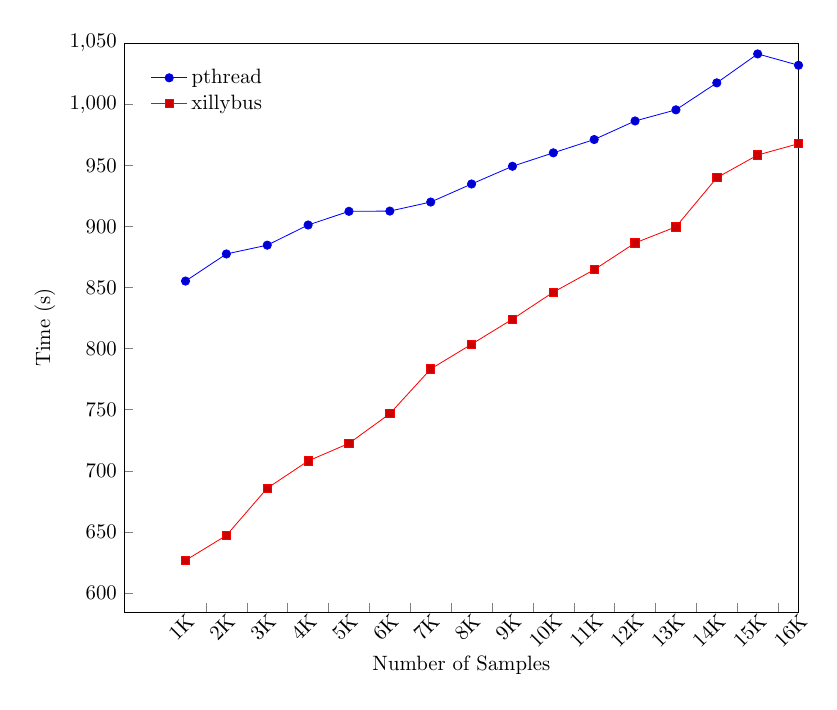
\begin{tikzpicture}[scale = 0.75]
	 \begin{axis}[
    	xlabel=Number of Samples,
		ylabel=Time ($\upmu$s),
	 	%scaled ticks=base 10:-5,
	 	xtick pos=left,
		ytick pos=left,
		ymax = 1050,
		xmax = 16384,
   		symbolic x coords={1024, 2048, 3072, 4096, 5120, 6144, 7168, 8192, 9216, 10240, 11264, 12288, 13312, 14336, 15360, 16384},
	 	xtick=data,
		xticklabels={1K, 2K, 3K, 4K, 5K, 6K, 7K, 8K, 9K, 10K, 11K, 12K, 13K, 14K, 15K, 16K},
	 	width = 13cm,
	 	xmode = normal,
	 	legend pos=north west,
	    legend style={draw=none},
	 	x tick label style={rotate=45, anchor=north east, inner sep=0mm},
		major x tick style = {opacity=0},
		minor x tick num = 1,
		minor tick length=1ex,
		every node near coord/.append style={
        anchor=west,
        rotate=90,
        font=\tiny
		},
	 ]    
   
	\addplot plot coordinates {
	    (1024,     855.3)
		(2048,     877.5)
		(3072,     884.7)
		(4096,     901.2)
		(5120,     912.4)
		(6144,     912.6)
		(7168,     920)
		(8192,     934.8)
		(9216,     949.3)
		(10240,    960.3)
		(11264,    971.2)
		(12288,    986.4)
		(13312,    995.5)
		(14336,    1017.6)
		(15360,    1041.3)
		(16384,    1032)
		};
    
	\addplot plot coordinates {
	    (1024,     626.6)
		(2048,     647)
		(3072,     685.7)
		(4096,     708)
		(5120,     722.4)
		(6144,     746.7)
		(7168,     783.3) 
		(8192,     803.6)
		(9216,     824.1)
		(10240,    846.2)
		(11264,    864.6)
		(12288,    886.5)
		(13312,    899.7)
		(14336,    939.9)
		(15360,    958.5)
		(16384,    967.8)
		};
		
    \legend{pthread\\xillybus\\} 
	\end{axis}
	\end{tikzpicture} 
	\label{writebuffer} 
	\caption{Timing Analysis for clEnqueueReadBuffer API} 
	\label{graph2:read}
\end{figure}